\documentclass{book}

\usepackage[utf8]{inputenc}
\usepackage[T1]{fontenc}
\usepackage[francais]{babel}
\usepackage{graphicx} 
\usepackage{fancyref}
\usepackage{hyperref}

\title{Classification d'images télévisées}
\author{\textsc{Farhad} - \textsc{Heybati}\\
\textsc{Youcef} - \textsc{Kacer}\\
\textsc{Martin} - \textsc{Provost}}
\date{9 May 2016}

\begin{document}
 
\maketitle

\tableofcontents

\frontmatter
\chapter{Introduction}
Ce document présente plusieurs méthodes d'extraction d'informations à partir d'images issues d'un débat télévisé.
Cela afin d'en effectuer une classification binaire en \og gros plan \fg{} ou \og large plan \fg{}.
Nous proposons dans un premier chapître de présenter les images exploitées, et les deux classes qui nous intéressent.
Dans une seconde partie, nous presentons les méthodes d'extraction d'informations utilisées.
Puis dans une troisième partie, les résultats obtenus.

\mainmatter
\chapter{Images exploitées}
\section{Corpus et labelisation}\label{labelisation}
Nous allons exploités un total de 2351 images prises à partir de la vidéo d'un débat télévisé \cite{ref} .
Nous avons exploité le fichier de transcription au format .trs \cite{ref} associé à cette vidéo, cela afin d'extraire les différents classes, et attribuer à chaque image sa classe.
En effet, le fichier de transcription fournit un total de 9 classes : \\


\begin{description} % listes descriptives

\item[$M$ :] La présentatrice est seule à l'écran
\item[$A$ :] La première intervenante est seule à l'écran
\item[$B$ :] La seconde intervenante est seule à l'écran
\item[$C$ :] Le premier intervenant est seul à l'écran
\item[$D$ :] Le second intervenant est seul à l'écran
\item[$ALL$ :] Les 5 personnes sont à l'écran
\item[$MULTI$ :] Entre 2 et 4 personnes sont à l'écran
\item[$INTRO$ :] Reportage d'introduction à l'écran
\item[$CREDITS$ :] Générique d'emission à l'écran\\

\end{description}

Par ailleurs, le fichier de transcription donne à chaque intervalle de temps, ce qui est à l'écran parmi les classes citées plus-haut. 
Moyennant un reformatage des données xml de ce fichier, on peut obtenir le tableau suivant :

\begin{table}[H]
\begin{center}
\begin{tabular}{|c|c|c|}
\hline
\begin{bf}classe\end{bf} & \begin{bf}debut (s)\end{bf} & \begin{bf}fin (s)\end{bf} \\
\hline
$CREDITS$	& 0 & 11.36 \\
\hline
$INTRO$   & 11.36	& 84.64 \\
\hline
$M$	& 84.64	& 95.12 \\
\hline
$ALL$	& 95.12	& 103.2 \\
\hline
$A$	& 103.2	& 112.2 \\
\hline
$M$	& 112.2	& 115.24 \\
\hline
\vdots & \vdots &\vdots \\
\hline
$M$	& 2334.12 & 2340 \\
\hline
$ALL$	& 2340 & 2340.76 \\
\hline
$CREDITS$	& 2340.76 & 2349.72 \\
\hline
\end{tabular}
\end{center}
\caption{Table de correspondance classes/intervalle de temps}
\label{Table correspondance classe/temps}
\end{table}
\clearpage

Les 2351 images étant prises à une seconde d'intervalle tout le long de la vidéo, on peut automatiquement labéliser celles ci via la table de
correspondance \ref{Table correspondance classe/temps}.
Ci-après, nous présentons quelques images pour chacune des 9 classes (Cf. figures \ref{classeM},\ref{classeA},\ref{classeB},\ref{classeC},\ref{classeD},
\ref{classeALL},\ref{classeMULTI},\ref{classeINTRO},\ref{classeCREDITS}).
\begin{figure}[H]
\begin{center}
\includegraphics[scale=0.3]{../data/frames/00000089.jpg}
\includegraphics[scale=0.3]{../data/frames/00000159.jpg}
\includegraphics[scale=0.3]{../data/frames/00000176.jpg}
\end{center}
\caption{image de classe $M$}
\label{classeM}
\end{figure}

\begin{figure}[H]
\begin{center}
\includegraphics[scale=0.3]{../data/frames/00000105.jpg}
\includegraphics[scale=0.3]{../data/frames/00000106.jpg}
\includegraphics[scale=0.3]{../data/frames/00000107.jpg}
\end{center}
\caption{image de classe $A$}
\label{classeA}
\end{figure}

\begin{figure}[H]
\begin{center}
\includegraphics[scale=0.3]{../data/frames/00000147.jpg}
\includegraphics[scale=0.3]{../data/frames/00000148.jpg}
\includegraphics[scale=0.3]{../data/frames/00000149.jpg}
\end{center}
\caption{image de classe $B$}
\label{classeB}
\end{figure}

\begin{figure}[H]
\begin{center}
\includegraphics[scale=0.3]{../data/frames/00000165.jpg}
\includegraphics[scale=0.3]{../data/frames/00000166.jpg}
\includegraphics[scale=0.3]{../data/frames/00000167.jpg}
\end{center}
\caption{image de classe $C$}
\label{classeC}
\end{figure}

\begin{figure}[H]
\begin{center}
\includegraphics[scale=0.3]{../data/frames/00000288.jpg}
\includegraphics[scale=0.3]{../data/frames/00000289.jpg}
\includegraphics[scale=0.3]{../data/frames/00000290.jpg}
\end{center}
\caption{image de classe $D$}
\label{classeD}
\end{figure}

\begin{figure}[H]
\begin{center}
\includegraphics[scale=0.3]{../data/frames/00000179.jpg}
\includegraphics[scale=0.3]{../data/frames/00000203.jpg}
\includegraphics[scale=0.3]{../data/frames/00000239.jpg}
\end{center}
\caption{image de classe $ALL$}
\label{classeALL}
\end{figure}

\begin{figure}[H]
\begin{center}
\includegraphics[scale=0.3]{../data/frames/00000213.jpg}
\includegraphics[scale=0.3]{../data/frames/00000251.jpg}
\includegraphics[scale=0.3]{../data/frames/00000310.jpg}
\end{center}
\caption{image de classe $MULTI$}
\label{classeMULTI}
\end{figure}

\begin{figure}[H]
\begin{center}
\includegraphics[scale=0.3]{../data/frames/00000013.jpg}
\includegraphics[scale=0.3]{../data/frames/00000024.jpg}
\includegraphics[scale=0.3]{../data/frames/00000041.jpg}
\end{center}
\caption{image de classe $INTRO$}
\label{classeINTRO}
\end{figure}

\begin{figure}[H]
\begin{center}
\includegraphics[scale=0.3]{../data/frames/00002344.jpg}
\includegraphics[scale=0.3]{../data/frames/00002348.jpg}
\includegraphics[scale=0.3]{../data/frames/00002350.jpg}
\end{center}
\caption{image de classe $CREDITS$}
\label{classeCREDITS}
\end{figure}

\section{Classification binaire}

Par la suite, nous allons nous resteindre à seulement deux classes définies comme suit :\\
\begin{description} % listes descriptives
\item[$G$ :] \og Gros plan \fg{} (une seule personne est à l'ecran)
\item[$L$ :] \og Large plan \fg{} (au moins deux personnes sont à l'écran)\\
\end{description}


Les classes $G$ et $L$ peuvent s'exprimer en fonction des 9 classes comme suit :\\

\begin{description} % listes descriptives
\item[$G$ :] $M$ | $A$ | $B$ | $C$ | $D$
\item[$L$ :] $ALL$ | $MULTI$\\
\end{description}


Nous avons donc deux classes d'images $G$ et $L$ (respectivement 1491 et 761 images) (Cf. figures \ref{classeG} et
\ref{classeL}) \\

\begin{figure}[H]
\begin{center}
\includegraphics[scale=0.2]{../data/frames/00000089.jpg}
\includegraphics[scale=0.2]{../data/frames/00000105.jpg}
\includegraphics[scale=0.2]{../data/frames/00000147.jpg}
\includegraphics[scale=0.2]{../data/frames/00000165.jpg}
\includegraphics[scale=0.2]{../data/frames/00000288.jpg}
\end{center}
\caption{image de classe $G$ (gros plan)}
\label{classeG}
\end{figure}

\begin{figure}[H]
\begin{center}
\includegraphics[scale=0.2]{../data/frames/00000336.jpg}
\includegraphics[scale=0.2]{../data/frames/00000394.jpg}
\includegraphics[scale=0.2]{../data/frames/00000458.jpg}
\includegraphics[scale=0.2]{../data/frames/00000474.jpg}
\includegraphics[scale=0.2]{../data/frames/00000625.jpg}
\end{center}
\caption{image de classe $L$ (large plan)}
\label{classeL}
\end{figure}

Par la suite, nous allons expliciter différentes manières d'extraire de l'information afin de pouvoir discriminer les images de classe $G$
, des images de classe $L$.

\chapter{Extraction d'information}
\section{Extraction de contours}

Cette méthode consiste à déterminer le nombre de contours détecté par des algorithmes de traitement
d'image contenu dans \begin{itshape}OpenCV\end{itshape}\cite{opencv_library}, et d'en déduire si l'image est un \og gros plan \fg{} ou un \og large plan \fg{}.\\
Nous effectuons 2 passes sur chaque image avec des paramétrages d'algorithmes différents afin de
produire 2 variables par image.\\
Dans chaque passe nous ajoutons un flou Gaussien à l'image afin d'atténuer les petits détails comme les
traits du visage ou du décor.\\
Ensuite, l'image est passée en niveau de gris pour être binarisée via un seuil adaptative ($\mathrm{cv::AdaptativeThreshold}$)\\
Et enfin, on execute la fonction ($\mathrm{cv::findContours}$) avec une option différente pour chaque passe.\\

La première passe extrait les contours avec l'option \begin{itshape}CHAIN\_APPRO\_NONE\end{itshape}. 
La seconde passe extrait les contours avec l'option \begin{itshape}CHAIN\_APPROX\_SIMPLE\end{itshape}. 

Les 2 informations du nombre de contours sont stockées ensuite dans un DataFrame comme descripteur
destiné à être classifié de manière supervisée.

\section{Extraction de saturation}
\subsection{Définition}
Hue, Saturation, Value ou HSV est un modèle qui représente la couleur (H) en fonction de la saturation (S) en gris et la luminosité (V) (Cf. figure \ref{HSV}).
\begin{figure}[H]
\begin{center}
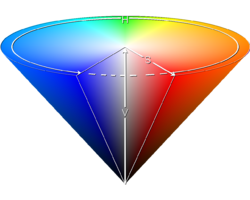
\includegraphics[scale=0.5]{hue.jpg}
\end{center}
\caption{Illustration $HSV$ \cite{wiki:hsv}}
\label{HSV}
\end{figure}
\begin{description}
\item[Teinte (Hue) :] Correspond à la couleur. Elle est définie sous la forme
d'un cercle où les trois couleurs primaires RVB sont
réparties aux angles 0\degre pour le rouge, 120\degre pour le vert
et 240\degre pour le bleu.
\item[Saturation :] C’est le taux de pureté de la couleur, qui varie entre un
maximale (couleur éclatante) et l’achromatisme (couleur
gris).
\item[Valeur :]  C’est la mesure de l’intensité lumineuse de la couleur
qui varie entre le noir et le blanc.
\end{description}

\subsection{Choix de la variable explicative}

Nous sommes partis de l’hypothèse que les images en \og gros plan \fg{} sont plutôt gris et donc une saturation en couleur plus faible que les images en \og large plan \fg{}.\\
La réalisation d’un histogramme sur la moyenne de saturation (Cf. Figure \ref{hue_histo}), portant sur la totalité des images, nous a permis d’identifier deux classes de type Gaussien pour modéliser nos 2 classes
qui sont les images de type \og gros plan \fg{} et les images de type \og large plan \fg{}\\
Nous présentons le code Python d'extraction de saturation et sa classification dans l'annexe \ref{code_python_saturation}
\label{hue_frontiere}
\begin{figure}[H]
\begin{center}
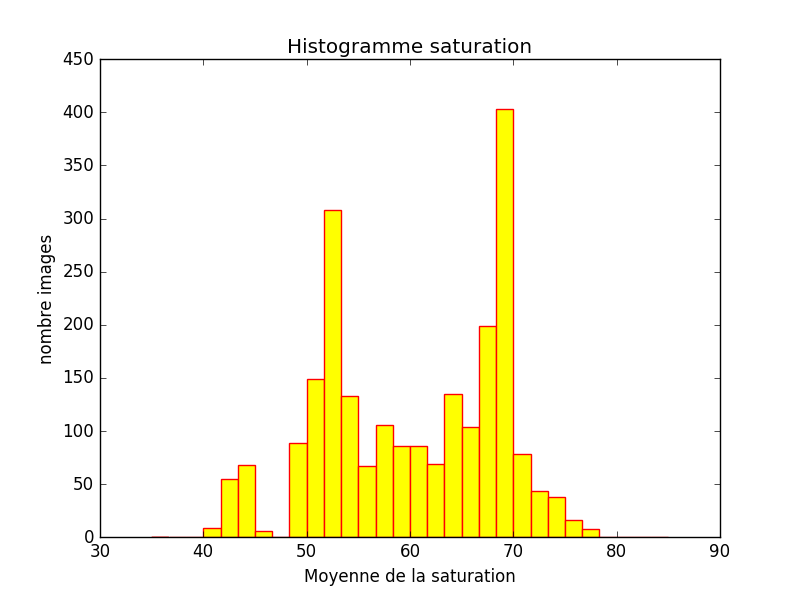
\includegraphics[scale=0.5]{hue_histogramme.jpg}
\end{center}
\caption{Histogramme des moyennes de saturation}
\label{hue_histo}
\end{figure}

La moyenne de la saturation globale obtenue est 60.2561640854. 
Nous avons considérés les images dont la saturation moyenne est inférieure à la moyenne globale comme appartenant à la classe \og gros plan \fg{} et les images dont 
la saturation moyenne est supérieure à la moyenne globale comme appartenant à la classe \og large plan \fg{}.

\section{Histogramme orienté du gradient}

Cette méthode consiste à extraire l'information local de contours. Historiquement, sa première utilisation a consisté en 
la détection de piétons \cite{hog}. Pour une image donnée, le vecteur descripteur des \begin{itshape}HOG\end{itshape} est la concaténation
d'histogrammes de l'amplitude du gradient (en fonction de son orientation). Chaque histogramme est pris sur un carré de l'image
appelé \og cellule \fg{}. L'ensemble des cellules quadrille entièrement l'image avec un eventuel recouvrement.\\
Ces histogrammes sont ensuite normalisés en intensité par paquet de cellules adjacentes (appelés \og block \fg{}) afin d'obtenir des descripteurs 
invariants au changement local d'illumination (Cf. figure \ref{hog}).
\begin{figure}[H]
\begin{center}
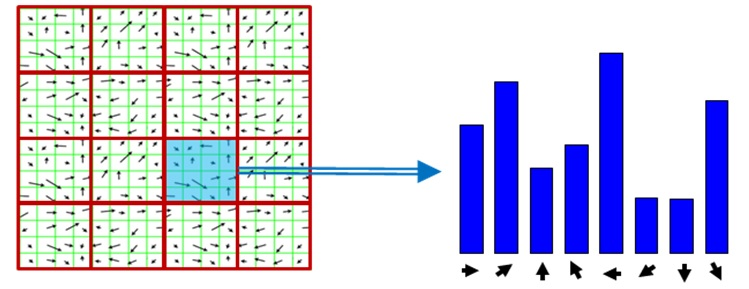
\includegraphics[scale=0.5]{hog.jpg}
\end{center}
\caption{Construction d'un histogramme orienté du gradient \cite{hog2}}
\label{hog}
\end{figure}

On peut espérer que ces descripteurs s'adaptent bien à notre problème. En effet, les epaules des intervenants à gauche 
et à droite de l'image, ainsi que leur visage, sont des contours descriminants pour la classe $G$ (gros plan)
(Cf. figure \ref{hog_classeG}). D'autre part, les gros plans ont un fond uniforme, 
ce qui donnera beaucoup de gradient nul, et donc un descripteur \begin{itshape}sparse\end{itshape} pour la classe $G$ (gros plan).

\begin{figure}[H]
\begin{center}
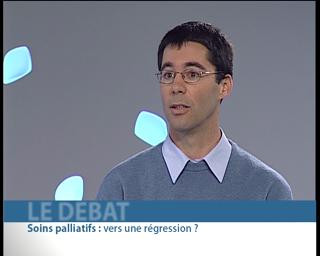
\includegraphics[scale=0.3]{hog_exemple.jpg}
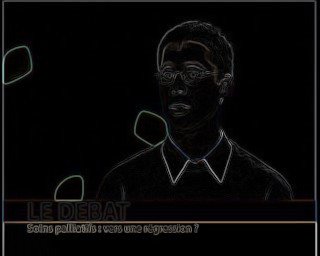
\includegraphics[scale=0.3]{hog_exemple_contour.jpg}
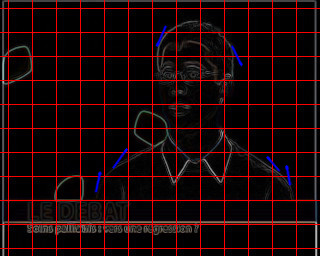
\includegraphics[scale=0.3]{hog_exemple_gradient.jpg}
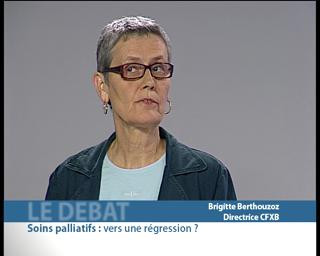
\includegraphics[scale=0.3]{hog_exemple2.jpg}
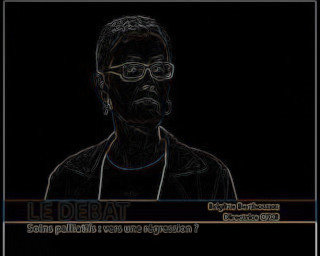
\includegraphics[scale=0.3]{hog_exemple2_contour.jpg}
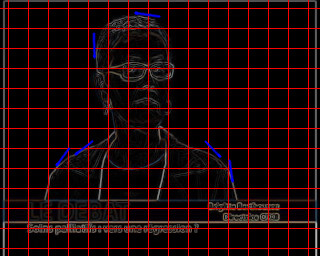
\includegraphics[scale=0.3]{hog_exemple2_gradient.jpg}
\end{center}
\caption{Histogramme orienté du gradient pour les gros plans (classe $G$)}
\label{hog_classeG}
\end{figure}

\section{Reseaux de neurones à convolution pré-entrainé}

Cette méthode consiste à extraire les descripteurs produits par un réseau de neurones à convolution déjà entrainé.
En effet, en récupérant la sortie de l'avant-dernière couche, on obtient la transformation finale haut-niveau de l'image, 
avant la couche de classification.
Cette technique est connue sous le nom de \begin{itshape}Transfer Learning\end{itshape} \cite{DBLP:journals/corr/YosinskiCBL14} 
et a fait ses preuves dans le cas de réseaux de neurones entrainé sur la base 
d'images \begin{itshape}ImageNet\end{itshape} \cite{imagenet_cvpr09}.
Cette base de près de 10 millions d'images, contient une multitude de classes (animaux,ustensiles,humains,...) organisées hiérarchiquement, 
et on peut espérer que les gros plans (classe $G$) correspondent à l'une de ces classes,et de même pour les images plan 
large (classe $L$), de telle sorte qu'on puisse ensuite séparer les descripteurs via un classifieur 
supervisé.

\chapter{Résultats}
\section{Extraction de contours}
Pour expliquer le résultat de l’extraction de contours, voici quelques exemples d'images où les contours ont été tracés avec 
la fonction $\mathrm{cv::drawContours}$.

La figure \ref{contouringG1} montrent deux exemples de contouring sur des images \og gros plan \fg{} (classe $G$), appliqué
avec l'option \begin{itshape}CHAIN\_APPRO\_NONE\end{itshape} (première passe)

\begin{figure}[H]
\begin{center}
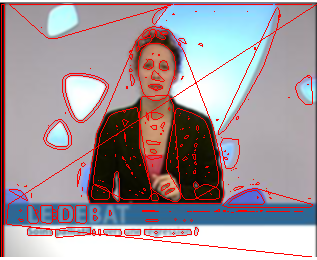
\includegraphics[scale=0.5]{contouring_exemple1_classeG_passe1.png}
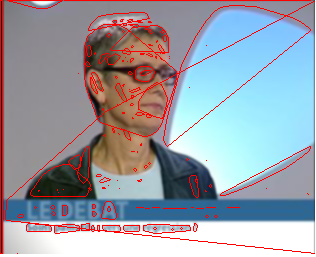
\includegraphics[scale=0.5]{contouring_exemple2_classeG_passe1.png}
\end{center}
\caption{Contouring sur des images de classe $G$ avec l'option CHAIN\_APPRO\_NONE}
\label{contouringG1}
\end{figure}

La figure \ref{contouringL1} montrent deux exemples de contouring sur des images \og large plan \fg{} (classe $L$), appliqué
avec l'option \begin{itshape}CHAIN\_APPRO\_NONE\end{itshape} (première passe)

\begin{figure}[H]
\begin{center}
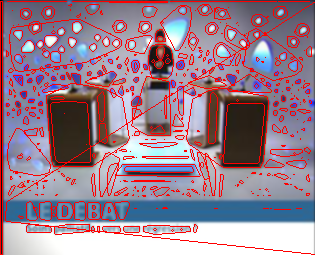
\includegraphics[scale=0.5]{contouring_exemple1_classeL_passe1.png}
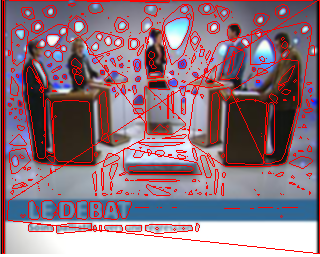
\includegraphics[scale=0.5]{contouring_exemple2_classeL_passe1.png}
\end{center}
\caption{Contouring sur des images de classe $L$ avec l'option CHAIN\_APPRO\_NONE}
\label{contouringL1}
\end{figure}

Il y a plus de contours dans les images \og large plan \fg{} car le décor du plateau TV est composé de beaucoup de détails.
Cela permet de bien différencier les gros plans des plans larges mais pour quelques cas le nombre de 
contours ne suffit pas.\\
Pour remédier à cela, nous avons mis en place la seconde passe et dont voici les résultats pour les mêmes 
images : 

La figure \ref{contouringG2} montre deux exemples de contouring sur des images \og gros plan \fg{} (classe $G$), appliqué
avec l'option \begin{itshape}CHAIN\_APPRO\_SIMPLE\end{itshape} (seconde passe).

La figure \ref{contouringL2} montre deux 
exemples de contouring sur des images \og large plan \fg{} (classe $L$), appliqué avec 
l'option \begin{itshape}CHAIN\_APPRO\_SIMPLE\end{itshape}\\


Le nombre de contours à beaucoup augmenté par rapport à la première passe, ce qui va permettre de différencier encore mieux 
les types de plans : en effet, on note ici un très grand nombre de contours dans le décor et sur les personnages, ce qui nous permet de 
mieux discriminer les plans larges.
Le bandeau du bas est plus détaillé en termes de contours que pour la première passe.

\begin{figure}[H]
\begin{center}
\includegraphics[scale=0.5]{contouring_exemple1_classeG_passe2.png}
\includegraphics[scale=0.5]{contouring_exemple2_classeG_passe2.png}
\end{center}
\caption{Contouring sur des images de classe $G$ avec l'option CHAIN\_APPRO\_SIMPLE}
\label{contouringG2}
\end{figure}

\begin{figure}[H]
\begin{center}
\includegraphics[scale=0.5]{contouring_exemple1_classeL_passe2.png}
\includegraphics[scale=0.5]{contouring_exemple2_classeL_passe2.png}
\end{center}
\caption{Contouring sur des images de classe $L$ avec l'option CHAIN\_APPRO\_SIMPLE}
\label{contouringL2}
\end{figure}

\section{Extraction de teinte}
En prenant comme frontière de décision, la valeur calculée en \ref{hue_frontiere}, alors on obtient un taux de prédiction correcte de 78.32\%.\\
Par ailleurs, nous avons demandé à différent classifieurs d'effectuer un apprentissage supervisé sur les moyennes de saturation. Pour cela, nous avons divisé les images
en deux sous-ensembles représentant 70\% du total pour l'entrainement, 30\% pour le test.\\
Les resultats de cette classification sont illustrés dans la table \ref{Table_resultats_hue}. On voit que SVM et Random Forest donnent des frontières plus complexes qui permettent
un meilleure score de test (90\%).\\
Les classifieurs utilisés sont ceux de la librairie \begin{itshape}Scikit-Learn\end{itshape}, implémentés dans le script 
\begin{itshape}Python\end{itshape} tiré de \cite{scikit_bench}, que nous avons adaptés.

\begin{table}
\begin{center}
\begin{tabular}{|p{5cm}|p{2cm}|p{2cm}|p{2cm}|}
\hline
\begin{bf}classifieur\end{bf}& \begin{bf}score de test\end{bf} & \begin{bf}temps de training (s)\end{bf} & \begin{bf}temps de test (s)\end{bf} \\
\hline
Ridge Classifier & 0.67 & 0.44 & 0.001\\
\hline
Perceptron &  0.652 & 0.005 & 0.0\\
\hline
Passive-Aggressive & 0.344 & 0.005 & 0.0\\
\hline
kNN & 0.779 & 0.002 & 0.003\\
\hline
Random forest & 0.906 & 0.421 & 0.021\\
\hline
linear SVM - L2 penalty & 0.630 & 0.002 & 0.0\\
\hline
SGDClassifier - L2 penalty & 0.655 & 0.003 & 0.0\\
\hline
linear SVM - L1 penalty	& 0.786 & 0.007 & 0.0\\
\hline
SGDClassifier - L1 penalty & 0.656 & 0.005 & 0.0\\
\hline
SGDClassifier - ElasticNet penalty & 0.616 & 0.005 & 0.0\\
\hline
NearestCentroid & 0.525 & 0.001 & 0.0\\
\hline
SVM & 0.902 & 0.215 & 0.062\\
\hline
linear SVM - L1 penalty - dual=False & 0.670 & 0.067 & 0.0\\
\hline
\end{tabular}
\end{center}
\caption{Résultats de classification supervisée sur les moyennes de saturation}
\label{Table_resultats_hue}
\end{table}

\section{Histogramme orienté du gradient}
Nous avons extrait les descripteurs \begin{itshape}HOG\end{itshape} pour chacune des images de classe $G$ et $L$, en utilisant 
une cellule de taille 32x32 (sans recouvrement) de sorte à récupérer les formes des épaules et du visage, et non les details 
plus petits liés au port de lunettes par exemple. Pour la normalisation, nous l'avons effectué par groupe de carré à 4 cellules (avec
recouvrement) afin de tenir compte du fait qu'au sein des gros plans, les intervenants peuvent être légèrement décalés.
Puis, nous avons appliquer à ces descripteurs, différent classifieurs supervisés. 
Nous avons découpé le set de descripteurs en deux sous-ensembles représentant 70\% du total pour l'entrainement, 
30\% pour le test. Les resultats de classification sont illustrés dans la table \ref{Table_resultats_hog}.\\
Les classifieurs utilisés sont ceux de la librairie \begin{itshape}Scikit-Learn\end{itshape}, implémentés dans le script 
\begin{itshape}Python\end{itshape} tiré de \cite{scikit_bench}, que nous avons adaptés.

\begin{table}
\begin{center}
\begin{tabular}{|p{5cm}|p{2cm}|p{2cm}|p{2cm}|}
\hline
\begin{bf}classifieur\end{bf}& \begin{bf}score de test\end{bf} & \begin{bf}temps de training (s)\end{bf} & \begin{bf}temps de test (s)\end{bf} \\
\hline
Ridge Classifier & 1.0 & 0.130 & 0.027\\
\hline
Perceptron & 1.0 & 0.219 & 0.028\\
\hline
Passive-Aggressive & 1.0 & 0.352 & 0.024\\
\hline
kNN & 0.998 & 0.221 & 2.875\\
\hline
Random forest & 1.0 & 1.321 & 0.012\\
\hline
linear SVM - L2 penalty & 1.0 & 0.197 & 0.024\\
\hline
SGDClassifier - L2 penalty & 1.0 & 0.202 & 0.024\\
\hline
linear SVM - L1 penalty & 1.0 & 0.283 & 0.024\\
\hline
SGDClassifier - L1 penalty & 1.0 & 0.634 & 0.024\\
\hline
SGDClassifier - ElasticNet penalty & 1.0 & 0.721 & 0.024\\
\hline
NearestCentroid & 0.996 & 0.049 & 0.028\\
\hline
SVM & 0.998 & 0.446 & 0.203\\
\hline
linear SVM - L1 penalty - dual=False & 1.0 & 0.238 & 0.003\\
\hline
\end{tabular}
\end{center}
\caption{Résultats de classification supervisée sur les descripteurs $HOG$}
\label{Table_resultats_hog}
\end{table}

\section{Reseaux de neurones à convolution pré-entrainé}
Nous avons utilisé le code \begin{itshape}Overfeat\end{itshape} \cite{DBLP:journals/corr/SermanetEZMFL13}, récupéré par clonage du dépôt 
Github correspondant \cite{overfeat}, pré-entrainé sur la base \begin{itshape}ImageNet\end{itshape} \cite{imagenet_cvpr09}.
Nous avons extrait les descripteurs pour chacune des images de classe $G$ et $L$ pour leur appliquer différent classifieurs
 supervisés. Nous avons découpé le set de descripteurs en deux sous-ensembles 70\% du total pour l'entrainement, 30\% pour le test.
 Les resultats de classification sont illustrés dans la table \ref{Table_resultats_overfeat}.\\
 Les classifieurs utilisés sont ceux de la librairie \begin{itshape}Scikit-Learn\end{itshape}, implémentés dans le script 
\begin{itshape}Python\end{itshape} tiré de \cite{scikit_bench}, que nous avons adaptés.

 
\begin{table}
\begin{center}
\begin{tabular}{|p{5cm}|p{2cm}|p{2cm}|p{2cm}|}
\hline
\begin{bf}classifieur\end{bf}& \begin{bf}score de test\end{bf} & \begin{bf}temps de training (s)\end{bf} & \begin{bf}temps de test (s)\end{bf} \\
\hline
Ridge Classifier & 1.0 & 0.762 & 0.152\\
\hline
Perceptron & 0.998 & 1.515 & 0.155\\
\hline
Passive-Aggressive & 1.0 & 1.852 & 0.150\\
\hline
kNN & 0.998 & 1.456 & 16.77\\
\hline
Random forest & 0.998 & 3.851 & 0.024\\
\hline
linear SVM - L2 penalty & 1.0 & 1.105 & 0.149\\
\hline
SGDClassifier - L2 penalty & 0.998 & 1.156 & 0.153\\
\hline
linear SVM - L1 penalty & 1.0 & 1.220 & 0.149\\
\hline
SGDClassifier - L1 penalty & 1.0 & 5.581 & 0.149\\
\hline
SGDClassifier - ElasticNet penalty & 1.0 & 6.062 & 0.151\\
\hline
NearestCentroid	& 0.987 & 0.302 & 0.221\\
\hline
SVM & 1.0 & 3.508 & 1.591\\
\hline
linear SVM - L1 penalty - dual=False & 1.0 & 1.150 & 0.011\\
\hline
\end{tabular}
\end{center}
\caption{Résultats de classification supervisée sur les descripteurs $Overfeat$}
\label{Table_resultats_overfeat}
\end{table}
\clearpage

\appendix
\chapter{Code Python pour l'extraction de saturation et sa classification}\label{code_python_saturation}
\begin{verbatim}
import numpy as np
import cv2
import os
import matplotlib.pyplot as plt
import shutil
import pandas as pd

saturation = []
path='c:/tmp/images_debat/'
dirs = os.listdir(path)
file_valid='c:/tmp/labels.csv'
# This would print all the files and directories
for file in dirs:
    if file.endswith((".jpg")):
        colorImage = cv2.imread(path+file)
        #print ('Traitement du fichier : ',path+file)
        rows, cols, nbChannels = colorImage.shape

        b,g,r = cv2.split(colorImage)
        colorImage=cv2.merge([r,g,b])
        color = ('b','g','r')
        clorImageHSV=cv2.cvtColor(colorImage, cv2.COLOR_BGR2HSV)
        h,s,v=cv2.split(clorImageHSV)
        sm=np.mean(s)
        saturation.append(sm)
        #if file == '00000108.jpg' or file == '00000110.jpg' or file == '00000147.jpg':
            #print ('saturation pour le fichier 108 - 110 -147:')
            #print sm

globalMean = np.mean(saturation)
print ('Moyenne globale:')
print globalMean
#print saturation
plt.hist(saturation, range = (35, 85), bins = 30, color = 'yellow',
            edgecolor = 'red')
plt.xlabel('Moyenne de la saturation')
plt.ylabel('nombre images')
plt.title('Histogramme saturation')
#hist=np.histogram(saturation)
#plt.bar(hist)
plt.show()
copyPathGrosPlan='c:/tmp/GrosPlan/'
copyPathLargePlan='c:/tmp/LargePlan/'
classif=pd.DataFrame(columns=('file_name', 'label'))
classif_multi=pd.DataFrame(columns=('file_name', 'sm'))
line = 0;
for file1 in dirs:
    if file1.endswith((".jpg")):
        colorImage = cv2.imread(path+file1)
        rows, cols, nbChannels = colorImage.shape

        r,g,b = cv2.split(colorImage)
        colorImage=cv2.merge([r,g,b])
        color = ('b','g','r')
        clorImageHSV=cv2.cvtColor(colorImage, cv2.COLOR_BGR2HSV)
        h,s,v=cv2.split(clorImageHSV)
        sm=np.mean(s)
        classif_multi.loc[line]=(file1,sm)
        #Gros plan
        if  sm <= (globalMean):
             classif.loc[line]=(file1,-1.)            
        #Large plan
        else:
            classif.loc[line]=(file1,1.)            
        
        line = line+1

classif.sort_values(['file_name'])
#print classif            
#Open the labelled file
labelfile = open(file_valid)
label_img = pd.read_csv(labelfile,sep=';', names=['file_name', 'label'],header=0,dtype={'label': float})
label_img.sort_values(['file_name'])
#print label_img

correct_predict = pd.merge(classif, label_img, on=['file_name', 'label'], how='inner')
#print len(correct_predict)
#print len(label_img)
print ('Resultat :', (float(len(correct_predict))/float(len(label_img)))*100.)
#print classif_multi
#print label_img
label_img_mrg = pd.merge(classif_multi, label_img, on=['file_name'], how='inner')
label_img_mrg = label_img_mrg.drop('file_name', 1)
#print label_img_mrg
label_img_mrg.to_csv('C:\perso\TP\Son-Image\classif_multi.csv', sep=';', encoding='utf-8')
\end{verbatim}

\backmatter

\listoftables

\listoffigures

\bibliographystyle{alpha}
\bibliography{biblio}

\end{document}